\documentclass[conference]{IEEEtran}
\IEEEoverridecommandlockouts
% The preceding line is only needed to identify funding in the first footnote. If that is unneeded, please comment it out.
\usepackage{cite}
\usepackage{amsmath,amssymb,amsfonts}
\usepackage{algorithmic}
\usepackage{graphicx}
\usepackage{textcomp}
\usepackage{xcolor}
\def\BibTeX{{\rm B\kern-.05em{\sc i\kern-.025em b}\kern-.08em
    T\kern-.1667em\lower.7ex\hbox{E}\kern-.125emX}}
\begin{document}

\title{ Low-Supply Voltage Sensor with an Optical Indicator: Design, Construction, and Analysis}

\author{\IEEEauthorblockN{1\textsuperscript{st} Miguel Villa Floran}
\IEEEauthorblockA{\textit{Computer Engineering Department} \\
\textit{California Polytechnic State University, San Luis Obispo}\\
San Luis Obispo, United States of America \\
miguel.villafloran@gmail.com}
}

\maketitle

\begin{abstract}
This experiment focuses on the design, construction, and analysis of a low-supply voltage sensor-indicator circuit employing a Zener diode based voltage limiter and LED indicator. Key components include a 4.3 V Zener diode, TLC3702 voltage comparator IC, and a multi-turn potentiometer. The circuit utilizes a linear voltage divider and Zener diode to monitor supply voltage, activating an LED when the voltage drops below a specified threshold. The experiment providing valuable insights into the functionality and performance of the designed circuit


\end{abstract}

\begin{IEEEkeywords}
Zener diode, voltage comparator, LED, linear voltage divider, voltage limiter
\end{IEEEkeywords}

\section{Introduction}

\subsection{Voltage Comparator}

The voltage comparator is a device that specializes in comparing the voltages of two incoming signals and producing a high or low output voltage to indicate which is larger. If the the voltage across the positive terminal $V_{in+}$ is greater than the voltage across the negative terminal $V_{in-}$, the voltage comparator generate a logical high output voltage $V_{DD}$. Otherwise, a logical low output voltage $V_{SS}$ is produced \cite{week6}.

The voltage comparator is utilized in this design to indicate whether the voltage supply drops below a specified threshold, which for our intents and purposes is 8 V.

\subsection{Voltage Limiting Zener Diode}
The Zener Diode exhibits similar behaviors and properties as the standard PN junction diode. However, Zener diodes are also designed to have a well-defined and sharp reverse breakdown voltage, also referred to as the Zener voltage ($V_z$). When a Zener diode connected across a circuit in reverse bias reaches its Zener voltage, it maintains its Zener voltage and behaves as a closed circuit regardless of current fluctuations and changes in voltage. It is safe to use a Zener Diode in breakdown so long as the power it dissipates is below its maximum power rating \cite{week7}.

\begin{figure}[htbp]
\centerline{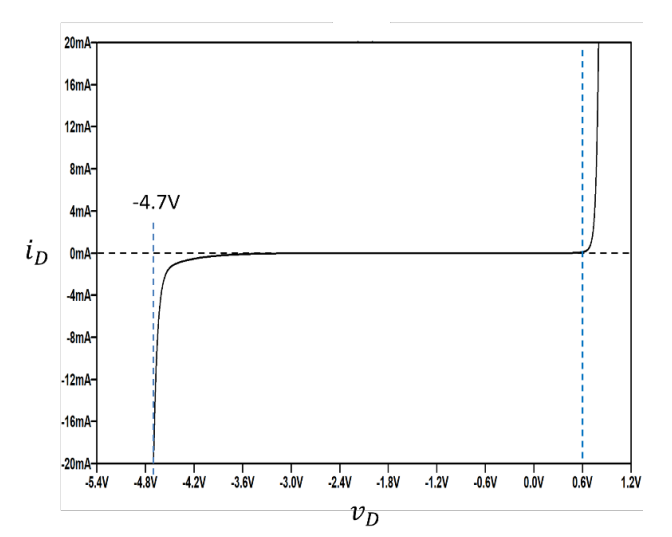
\includegraphics{./images/vi-characteristics.png}}
\caption{VI Characteristic of the 4.3V Zener Diode. \cite{week7}}
\label{fig}
\end{figure}

The reverse breakdown properties of a Zener Diode are leveraged to create voltage limiters for regulating the voltage across sensitive components or provide constant reference voltages \cite{week7}. This is done by connecting a resistor, which limits the current coming into the diode, in series to the Zener Diode, which is connected in parallel to the load. In this design, the Zener Diode provides a constant voltage across the negative terminal of the comparator \eqref{eq_1}.

\begin{equation}
V_- \approx V_Z\label{eq_1}
\end{equation}


\subsection{Multi-Turn Potentiometer}

A multi-turn rotary potentiometer is a type of voltage divider whose resistance changes as it is rotated, allowing for variable control of the output voltage in electronic circuits. The 

This adjustable resistance is utilized in this circuit so that the positive terminal's voltage is equivalent to the negative terminal's voltage, which is equivalent to the Zener voltage so that the comparator is tripped at the threshold voltage. The values of the potentiometer can also be found mathematically by using \eqref{eq_3}, but was found experimentally.

\begin{equation}
V_+ = \frac{R_a}{R_a + R_b} V_{DD}\label{eq_2}
\end{equation}

\begin{equation}
V_{DD(trip)} = (1 + \frac{R_b}{R_a})V_{Z}\label{eq_3}
\end{equation}

\subsection{LED Optical Indicator}

The light-emitting diode (LED) indicator serves as a visual cue, activating when the supply voltage falls below the predetermined threshold. The LED is reverse-biased relative to the output of the comparator and its cathode is connected to the supply voltage to ensure it only lights up when the supply voltage drops below the threshold voltage. When the supply voltage is above the threshold voltage, the comparator outputs the supply voltage, and the LED does not activate as there is no potential difference across it. When the supply voltage is below the threshold voltage, the comparator outputs 0 V, and the LED activates as there is a potential difference across it. To ensure the LED does not burn out, a resistor is added to limit current coming into the LED. This resistance is found by using \eqref{eq_3}, where 

and the rated forward current of the LED and the low current rating of the comparator.

\begin{equation}
R_{LED} \approx \frac{V_{DD(trip)} - V_{LED}}{I_{LED}}\label{eq_4}
\end{equation}

\section{Sensor Test and Data}

This experiment required a single circuit to be assembled in three phases to ensure its proper functionality and performance. In the initial phase, the voltage limiter is assembled to validate the biasing and behavior the Zener-based limiter. In the second phase, the Zener diode (D1) is integrated to create the voltage limiter. The Zener diode is connected in reverse bias across the supply voltage, and its breakdown characteristics are leveraged to maintain a stable reference voltage. The LED (LED1) is not yet included in this phase.

. The Zener diode selected for the voltage limiter is a 4.3V Zener diode, providing a stable reference voltage for the circuit. A multi-turn potentiometer is employed to set the desired threshold voltage at which the LED indicator is activated.

\subsection{Circuit Design}

The circuit design involves the integration of the voltage comparator, Zener diode, and potentiometer to create a low-supply voltage sensor with an optical indicator. The primary components include a 4.3V Zener diode (D1), TLC3702 voltage comparator IC (U1), LED indicator (LED1), and a multi-turn potentiometer (R1).

The voltage divider network consists of resistors R2 and R3, setting the threshold voltage at the non-inverting input ($V_{in+}$) of the voltage comparator. The Zener diode (D1) and resistor R4 form a Zener voltage limiter to monitor the supply voltage ($V_{in}$). The LED (LED1) is activated when the voltage falls below the specified threshold.

The potentiometer (R1) is employed to adjust the reference voltage at the inverting input ($V_{in-}$) of the voltage comparator, setting the threshold for activation. This adjustable feature enhances the flexibility of the sensor, allowing users to customize the trigger voltage according to specific requirements.

4.3V Zener diode, TLC3702 voltage comparator IC, and a multi-turn potentiometer


the biasing tail current IEE was implemented using
the LM334, an IC based current source. The value of Rset was
calculated using the data-sheet and is 330Ω. Rc1 and Rc2 in
figure 1 are the same as R in figure 2. These resistor values
are all 24kΩ. Lastly, VCC and VEE are connected to +5V and
-5V.
The resistive loaded differential pair has two outputs labeled, out1 and out2. Regarding in1, out2 is the non-inverting
output of this differential pair. Out1 can also be used as an
inverting output if needed. For this experiment, all data was
taken from the non-inverting side out2.
The actively loaded differential pair has only one output. A
current mirror helps distribute the current in each transistor.
Thus, the diode connected transistor in the current mirror will
have a small collector-emitter resistance so the performance
of the current mirror can be easily degraded. Similar to the
resistive loaded differential pair, the right side output is also
a non-inverting output for the actively loaded differential pair



. The first phase involved the assembly of the Zener diode based voltage limiter. The second phase involved the assembly of the linear voltage divider. The third phase involved the assembly of the voltage comparator. The circuit was assembled and tested using the following components:


and tested at 

igure 3: Schematics illustrating the recommended step-by-step assembly and testing of the low-supply voltage circuit: 
(a) biasing and verification of the Zener-based limiter; (b) adjustment of the linear voltage divider ensuring near zero 
voltage difference at the desired trip voltage of 8V; (c) verification that the comparator switches states at 
approximately 8V;

This experiment required three different circuits to be assembled and tested shown in figures \ref{circuit1}, \ref{circuit2}, and \ref{circuit3}. For all circuits, the biasing tail current IEE was implemented using the LM334, an IC based current source. The value of Rset was calculated using the data-sheet and is 330Ω. Rc1 and Rc2 in figure 1 are the same as R in figure 2. These resistor values are all 24kΩ. Lastly, VCC and VEE are connected to +5V and -5V.

\begin{figure}[htbp]
\centerline{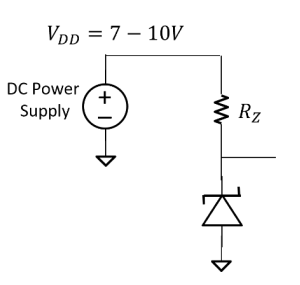
\includegraphics{./images/circuit1.png}}
\caption{Schematic with the Zener-based limiter assembled. \cite{week7}}
\label{circuit1}
\end{figure}

\begin{figure}[htbp]
\centerline{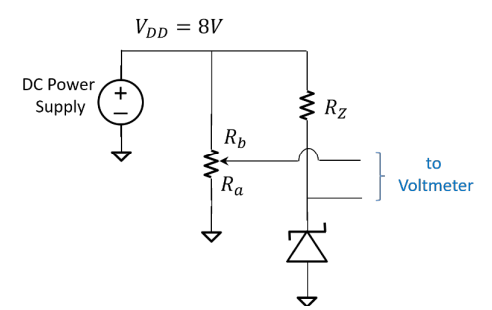
\includegraphics{./images/circuit2.png}}
\caption{Schematic assembled to fine-tune the potentiometer's value until the voltage difference at the trip voltage is close to zero. \cite{week7}}
\label{circuit2}
\end{figure}

\begin{figure}[htbp]
\centerline{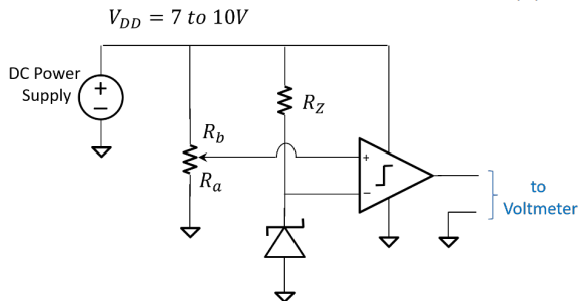
\includegraphics{./images/circuit3.png}}
\caption{Schematic assembled to verifiy that the comparator switches states at the specified trip voltage. \cite{b2}}
\label{circuit3}
\end{figure}

Before you begin to format your paper, first write and save the content as a 
separate text file. Complete all content and organizational editing before 
formatting. Please note sections \ref{AA}--\ref{SCM} below for more information on 
proofreading, spelling and grammar.

Keep your text and graphic files separate until after the text has been 
formatted and styled. Do not number text heads---{\LaTeX} will do that 
for you.

\subsection{Abbreviations and Acronyms}\label{AA}
Define abbreviations and acronyms the first time they are used in the text, 
even after they have been defined in the abstract. Abbreviations such as 
IEEE, SI, MKS, CGS, ac, dc, and rms do not have to be defined. Do not use 
abbreviations in the title or heads unless they are unavoidable.

\subsection{Units}
\begin{itemize}
\item Use either SI (MKS) or CGS as primary units. (SI units are encouraged.) English units may be used as secondary units (in parentheses). An exception would be the use of English units as identifiers in trade, such as ``3.5-inch disk drive''.
\item Avoid combining SI and CGS units, such as current in amperes and magnetic field in oersteds. This often leads to confusion because equations do not balance dimensionally. If you must use mixed units, clearly state the units for each quantity that you use in an equation.
\item Do not mix complete spellings and abbreviations of units: ``Wb/m\textsuperscript{2}'' or ``webers per square meter'', not ``webers/m\textsuperscript{2}''. Spell out units when they appear in text: ``. . . a few henries'', not ``. . . a few H''.
\item Use a zero before decimal points: ``0.25'', not ``.25''. Use ``cm\textsuperscript{3}'', not ``cc''.)
\end{itemize}

\subsection{Equations}
Number equations consecutively. To make your 
equations more compact, you may use the solidus (~/~), the exp function, or 
appropriate exponents. Italicize Roman symbols for quantities and variables, 
but not Greek symbols. Use a long dash rather than a hyphen for a minus 
sign. Punctuate equations with commas or periods when they are part of a 
sentence, as in:
\begin{equation}
a+b=\gamma\label{eq}
\end{equation}

Be sure that the 
symbols in your equation have been defined before or immediately following 
the equation. Use ``\eqref{eq}'', not ``Eq.~\eqref{eq}'' or ``equation \eqref{eq}'', except at 
the beginning of a sentence: ``Equation \eqref{eq} is . . .''

\subsection{\LaTeX-Specific Advice}

Please use ``soft'' (e.g., \verb|\eqref{Eq}|) cross references instead
of ``hard'' references (e.g., \verb|(1)|). That will make it possible
to combine sections, add equations, or change the order of figures or
citations without having to go through the file line by line.

Please don't use the \verb|{eqnarray}| equation environment. Use
\verb|{align}| or \verb|{IEEEeqnarray}| instead. The \verb|{eqnarray}|
environment leaves unsightly spaces around relation symbols.

Please note that the \verb|{subequations}| environment in {\LaTeX}
will increment the main equation counter even when there are no
equation numbers displayed. If you forget that, you might write an
article in which the equation numbers skip from (17) to (20), causing
the copy editors to wonder if you've discovered a new method of
counting.

{\BibTeX} does not work by magic. It doesn't get the bibliographic
data from thin air but from .bib files. If you use {\BibTeX} to produce a
bibliography you must send the .bib files. 

{\LaTeX} can't read your mind. If you assign the same label to a
subsubsection and a table, you might find that Table I has been cross
referenced as Table IV-B3. 

{\LaTeX} does not have precognitive abilities. If you put a
\verb|\label| command before the command that updates the counter it's
supposed to be using, the label will pick up the last counter to be
cross referenced instead. In particular, a \verb|\label| command
should not go before the caption of a figure or a table.

Do not use \verb|\nonumber| inside the \verb|{array}| environment. It
will not stop equation numbers inside \verb|{array}| (there won't be
any anyway) and it might stop a wanted equation number in the
surrounding equation.

\subsection{Some Common Mistakes}\label{SCM}
\begin{itemize}
\item The word ``data'' is plural, not singular.
\item The subscript for the permeability of vacuum $\mu_{0}$, and other common scientific constants, is zero with subscript formatting, not a lowercase letter ``o''.
\item In American English, commas, semicolons, periods, question and exclamation marks are located within quotation marks only when a complete thought or name is cited, such as a title or full quotation. When quotation marks are used, instead of a bold or italic typeface, to highlight a word or phrase, punctuation should appear outside of the quotation marks. A parenthetical phrase or statement at the end of a sentence is punctuated outside of the closing parenthesis (like this). (A parenthetical sentence is punctuated within the parentheses.)
\item A graph within a graph is an ``inset'', not an ``insert''. The word alternatively is preferred to the word ``alternately'' (unless you really mean something that alternates).
\item Do not use the word ``essentially'' to mean ``approximately'' or ``effectively''.
\item In your paper title, if the words ``that uses'' can accurately replace the word ``using'', capitalize the ``u''; if not, keep using lower-cased.
\item Be aware of the different meanings of the homophones ``affect'' and ``effect'', ``complement'' and ``compliment'', ``discreet'' and ``discrete'', ``principal'' and ``principle''.
\item Do not confuse ``imply'' and ``infer''.
\item The prefix ``non'' is not a word; it should be joined to the word it modifies, usually without a hyphen.
\item There is no period after the ``et'' in the Latin abbreviation ``et al.''.
\item The abbreviation ``i.e.'' means ``that is'', and the abbreviation ``e.g.'' means ``for example''.
\end{itemize}
An excellent style manual for science writers is \cite{b7}.

\subsection{Authors and Affiliations}
\textbf{The class file is designed for, but not limited to, six authors.} A 
minimum of one author is required for all conference articles. Author names 
should be listed starting from left to right and then moving down to the 
next line. This is the author sequence that will be used in future citations 
and by indexing services. Names should not be listed in columns nor group by 
affiliation. Please keep your affiliations as succinct as possible (for 
example, do not differentiate among departments of the same organization).

\subsection{Identify the Headings}
Headings, or heads, are organizational devices that guide the reader through 
your paper. There are two types: component heads and text heads.

Component heads identify the different components of your paper and are not 
topically subordinate to each other. Examples include Acknowledgments and 
References and, for these, the correct style to use is ``Heading 5''. Use 
``figure caption'' for your Figure captions, and ``table head'' for your 
table title. Run-in heads, such as ``Abstract'', will require you to apply a 
style (in this case, italic) in addition to the style provided by the drop 
down menu to differentiate the head from the text.

Text heads organize the topics on a relational, hierarchical basis. For 
example, the paper title is the primary text head because all subsequent 
material relates and elaborates on this one topic. If there are two or more 
sub-topics, the next level head (uppercase Roman numerals) should be used 
and, conversely, if there are not at least two sub-topics, then no subheads 
should be introduced.

\subsection{Figures and Tables}
\paragraph{Positioning Figures and Tables} Place figures and tables at the top and 
bottom of columns. Avoid placing them in the middle of columns. Large 
figures and tables may span across both columns. Figure captions should be 
below the figures; table heads should appear above the tables. Insert 
figures and tables after they are cited in the text. Use the abbreviation 
``Fig.~\ref{fig}'', even at the beginning of a sentence.

\begin{table}[htbp]
\caption{Table Type Styles}
\begin{center}
\begin{tabular}{|c|c|c|c|}
\hline
\textbf{Table}&\multicolumn{3}{|c|}{\textbf{Table Column Head}} \\
\cline{2-4} 
\textbf{Head} & \textbf{\textit{Table column subhead}}& \textbf{\textit{Subhead}}& \textbf{\textit{Subhead}} \\
\hline
copy& More table copy$^{\mathrm{a}}$& &  \\
\hline
\multicolumn{4}{l}{$^{\mathrm{a}}$Sample of a Table footnote.}
\end{tabular}
\label{tab1}
\end{center}
\end{table}

\begin{figure}[htbp]
\centerline{\includegraphics{images/fig1.png}}
\caption{Example of a figure caption.}
\label{fig}
\end{figure}

Figure Labels: Use 8 point Times New Roman for Figure labels. Use words 
rather than symbols or abbreviations when writing Figure axis labels to 
avoid confusing the reader. As an example, write the quantity 
``Magnetization'', or ``Magnetization, M'', not just ``M''. If including 
units in the label, present them within parentheses. Do not label axes only 
with units. In the example, write ``Magnetization (A/m)'' or ``Magnetization 
\{A[m(1)]\}'', not just ``A/m''. Do not label axes with a ratio of 
quantities and units. For example, write ``Temperature (K)'', not 
``Temperature/K''.

\begin{thebibliography}{00}
\bibitem{week6} Week 6: Elementary Logic Circuits - Part II, Available https://canvas.calpoly.edu/courses/113173/files?preview=11616452
\bibitem{week7} Week 7: A Low-Supply Voltage Sensor with an Optical Indicator, Available https://canvas.calpoly.edu/courses/113173/files?preview=11699080
\bibitem{b2} M. Shell, ``How to Use the IEEEtran \LaTeX Class,`` IEEE Transactions on Professional Communication, vol. PP, no. 99, pp. 1-1, 20XX. [Online]. Available: http://www.michaelshell.org/
\end{thebibliography}
\vspace{12pt}

\end{document}
